%%% Plantilla creada para Proyecto de Investigación
%%% del Bachillerato de Excelencia, IES San Mateo, Madrid
%%% Por Roberto Rodríguez del Río 
%%% rrdelrio@ucm.es
%%% Ver 1.0, Junio 2016
\documentclass[a4paper,12pt]{article} 

\usepackage[utf8]{inputenc}
\usepackage[spanish]{babel}
\usepackage{amsmath}
\usepackage{amsfonts}
\usepackage{amssymb} 

\usepackage{graphicx} 
\usepackage{hyperref} 
\usepackage{wrapfig}
\usepackage{enumitem}
\usepackage{fancyhdr}
\usepackage{float}
\usepackage{eurosym}
\usepackage{color}
\usepackage{titling}
\usepackage{lipsum}
\usepackage{tocbibind}
\usepackage{xcolor}
\usepackage{listings}
\usepackage{etoolbox}
\usepackage{float}
\usepackage{atbegshi}% http://ctan.org/pkg/atbegshi
\AtBeginDocument{\AtBeginShipoutNext{\AtBeginShipoutDiscard}}


\usepackage[left=3cm,right=3cm,top=3cm,bottom=4cm]{geometry}


\pagestyle{fancy}


%%% Para las cabeceras
\newcommand{\hsp}{\hspace{20pt}}
\newcommand{\HRule}{\rule{\linewidth}{0.5mm}}
\headheight=50pt
%%% 
\newcommand{\vacio}{\textcolor{white}{holacaracola}}

%%% Para que las ecuaciones se numeren
%%% con el número de sección y el de ecuación.
\renewcommand{\theequation}{\thesection.\arabic{equation}}


% Color azul para algunos 
% textos de la portada
\definecolor{azulportada}{rgb}{0.16, 0.32, 0.75}

%%%% Azul para textos de headings
\definecolor{azulinterior}{rgb}{0.0, 0.2, 0.6}

%%%%%%%%defniciones para codigo

\definecolor{mygreen}{rgb}{0,0.6,0}
\definecolor{mygray}{rgb}{0.5,0.5,0.5}
\definecolor{mymauve}{rgb}{0.58,0,0.82}
\definecolor{blueviolet}{rgb}{0.54,0.17,0.89}
\definecolor{Decorators}{rgb}{0.7,0,0.7}
\definecolor{self}{rgb}{.87,.46,0}
\definecolor{classname}{RGB}{101,0,67}
\definecolor{methodname}{RGB}{4,7,98}
\definecolor{characters}{RGB}{171,122,8}

\maxdeadcycles=1000
\extrafloats{100}

\makeatletter
\lstset{ %
  frame=lines,
  showlines=true,
  showstringspaces=false, 
  breaklines=true,
  columns=fullflexible
  tabsize=4,
  basicstyle=\ttfamily\small,
  backgroundcolor=\color{white},   % choose the background color
  basicstyle=\footnotesize,        % size of fonts used for the code
  breaklines=true,                 % automatic line breaking only at whitespace
  captionpos=b,                    % sets the caption-position to bottom
  commentstyle=\color{mygreen},    % comment style
  escapeinside={\%*}{*)},          % if you want to add LaTeX within your code
  keywordstyle=\color{blue},       % keyword style
  stringstyle=\color{mymauve},     % string literal style
  literate={á}{{\'a}}1 {ã}{{\~a}}1 {é}{{\'e}}1 {í}{{\'i}}1 {ó}{{\'o}}1 {ú}{{\'u}}1,  
  % additional keywords
  keywordstyle={[2]\color{Decorators}},
  emph={self},
  emphstyle={\color{self}\slshape},
  emph={[2]{__init__}},
  emphstyle=[2]{\color{blueviolet}\slshape},
  emph={[2]{__init__, __doc__}},
  emphstyle=[2]{\color{blueviolet}\slshape},
  emph={[3]{RelationModel, IrreducibleFD, CandidatesKeys}},
  emphstyle=[3]{\color{classname}\slshape},
  emph={[4]{saveAsJson, loadSetsFromJson, __convertListToSets, calculateAttributeClosure, calculateAttributeClosure2, checkEquivalenceJson, checkEquivalence, __generateFDfromFD, saveIrreducibleFD, __calculateCanonicalCover, __validateDependencies, __setOneAttributeRight, __setIrreducibleAttributeLeft, __deleteExtraneousAttributes, __deleteRedundantFD, setAttributeSets, checkPrimaryKey, calculateCandidateKeys, getKeysAtLevel, checkIsSupperKey}},
  emphstyle=[4]{\color{methodname}\slshape},
  emph={[5]{as}},
  emphstyle=[5]{\color{blue}\slshape},
}


\pretocmd\lst@makecaption{\noindent{\rule{\linewidth}{2pt}}}{}{}
\makeatother

\makeatletter
\patchcmd{\@makecaption}
  {\scshape}
  {}
  {}
  {}
\makeatother

\makeatletter
\patchcmd{\@makecaption}
  {\\}
  {.\ }
  {}
  {}
\makeatother

\renewcommand{\lstlistingname}{Programa}% Listing -> Programa


%%%%%%%%%%%%%%%
%%%%%%%%%%%%%%%%%%%%%%%
%%%%%%%%%salida de consola%%%%%%%%%%

%%%%%%%%%%%%%%%%%%%%%%%%%

%%%%%%%%%%%%%%%%%%%%%%%%%%%%%%%%
%%%%%% Datos del proyecto %%%%%%
%%%%%%%%%%%%%%%%%%%%%%%%%%%%%%%%
%%%TÍTULO
%%% Escribirlo en minúsculas, el programa
%%% lo pondrá en mayúsculas en la portada.
\title{Manual del Usuario}
%%%% AUTOR
\author{Laura Camila Scarpetta Rodríguez \\
		\texttt{20172495016} \\
		José Manuel Vargas Montero \\
		\texttt{20172495017}}
%%%%%%%%%%%%%%%%
%%%%%% DIRECTOR DEL TRABAJO
%%%%%%% Cambiar el nombre siguiente
\newcommand{\director}{Roberto Pava Díaz }
%%%%%%%%%%%%%%%

%%%%%%%%%%%%%%%%%%%%%
%%%%%%%%%%%%%%%%%%%%
\begin{document}

%%%%%%%%%%%%%%%%%%%%%%%%%%%%%%%
%%%%%%%%%%%%%%%%%%%%%%%%%%%%%%%
\begin{titlepage} %%%%% Aquí no hay que tocar nada.
	%%%% Las siguientes instrucciones generarán automáticamente
	%%%% la portada de tu proyecto.
	%%% Cambio de la estructura de esta página
\newgeometry{left=0.6cm,top=1.3cm,bottom=1.2cm}

\fbox{\parbox[c]{18.5cm}{
\begin{center}
\vspace{1.5cm}
{\fontfamily{phv}\fontsize{24}{6}\selectfont{Universidad Distrital Francisco José de Caldas}}\\
[1em]
{\fontfamily{phv}\fontsize{16}{5}\selectfont{Maestría en Ciencias de la Información y la Comunicación}}\\
[1em]
{\fontfamily{phv}\fontsize{26}{5}\selectfont{BASES DE DATOS}}\\
[2.6cm]
% Autor del trabajo de investigación
\textcolor{azulportada}{\fontfamily{phv}\fontsize{16}{5}\selectfont{\theauthor}}\\
[1cm]
% Título del trabajo
\textcolor{azulportada}
{\fontfamily{phv}\fontsize{30}{5}\selectfont{\textsc{\thetitle}}}\\
%{\Huge\textbf{\thetitle}}\\
[1cm]

\includegraphics[width=5.5cm]{Images/ud_escudo.png}
\\[2cm]
{\fontfamily{phv}\fontsize{16}{5}\selectfont{Docente}}\\
[0.5cm]
{\fontfamily{phv}\fontsize{16}{5}\selectfont{\director}}\\
[2cm]
{\fontfamily{phv}\fontsize{16}{5}\selectfont{\today}}\\
[4cm]
\end{center}
}}
 
 \restoregeometry
 %%%% Volvemos a la estructura de la página normal

\end{titlepage}

%%%%%%%%%%%%%%%%%%%%%%%%%%%%%%

{%\Large

\newpage

%%%Encabezamiento y pie de página
%%% También se genera automáticamente
%%% Mejor no tocarlo mucho.
\renewcommand{\headrulewidth}{0.5pt}
\fancyhead[R]{
	\textcolor{azulinterior}{\fontfamily{phv}\fontsize{14}{4}\selectfont{\textbf{\thetitle}}}\\
{\fontfamily{phv}\fontsize{10}{3}\selectfont{\theauthor}}}
\fancyhead[L]{\vacio}

\renewcommand{\footrulewidth}{0.5pt}
\fancyfoot[L]{\footnotesize Maestría en Ciencias de la Información y la Comunicación --- Bases de Datos}
\fancyfoot[C]{}
\fancyfoot[R]{\footnotesize Página \thepage}


%%%%%%%%%%%%%%%%%%%%

\

\vacio

\


\subsection*{Resumen}
En el presente informe encontrará un algoritmo que partiendo de una relación, con el conjunto de atributos $T$ y el de dependencias funcionales $L$, determinará si está en segunda forma normal, tercera o forma de Boyce-Codd.


\subsection*{Abstract}
\textsl{
In the present report it is pretended to develop an algortih which is able to determine whether the set of candidate keys from a Relation with its attributes set $T$ and functional dependencies $L$ is in first normal form, second one or Boyce-Codd.}

\ %% Así hago que se abra más espacio entre renglones.

\

\hrule

\

\


\paragraph{Palabras clave:} Dependencia funcional, conjuntos, llave candidata, llave primaria, formas normales.

\


\paragraph{Keywords:} Functional dependence, sets, candidate key, primary key, normal forms.







\newpage

%%% En esta página va el índice,
%%% pero no hay que hacer nada porque 
%%% se generará automáticamente.

\tableofcontents

\newpage



\section{Requerimientos}
\begin{enumerate}
\item Taller 2 Finalizado.
\item Implementar una interfaz gráfica Usable.
\end{enumerate}

\section{Notas}

\begin{enumerate}
\item Actividad en grupos de máximo (4)  integrantes.
\begin{enumerate}
\item Nombre, código y Número de lista
\item Un solo integrante realiza el envío en el aula virtual.
\end{enumerate}
\item Formato de entrega: 
\begin{enumerate}
\item Documento PDF.
\begin{enumerate}
\item Manual de Usuario.
\end{enumerate}
\item Código fuente: URL repositorio de código fuente.
\end{enumerate}
\end{enumerate}

\section{Solución}

\subsection{Herramienta tecnológica}
Para la solución del problema se decidió hacer uso del lenguaje de programación de Python. Para ello se utilizó el objeto set que Python tiene incorporada para trabajar conjuntos. Se utilizó PyCharm Community Edition 2018 como entorno de desarrollo, ya que las anteriores nos facilitan llegar a la solución del problema. 


\subsection{Interfaz Gráfica}

Se explica el correcto uso de la interfaz gráfica.\\

\subsubsection{Formato del archivo JSON}

Esta interfaz permite cargar los datos provenientes de un archivo JSON. 
\\
Dicho archivo debe tener el siguiente formato:

\begin{lstlisting}[language=python, caption={Archivo JSON de relación de ejemplo.\\\hspace{\textwidth}}, captionpos=t]
{"t_set": ["A", "B", "C", "D", "E"], "l_set": [["ABC", "D"], ["D", "A"]]}
\end{lstlisting}

Esto es vital para el correcto funcionamiento de la interfaz gráfica.

\subsubsection{Inicio}

Al iniciar la interfaz gráfica se observará lo siguiente:

\begin{figure}[H]
\centering
  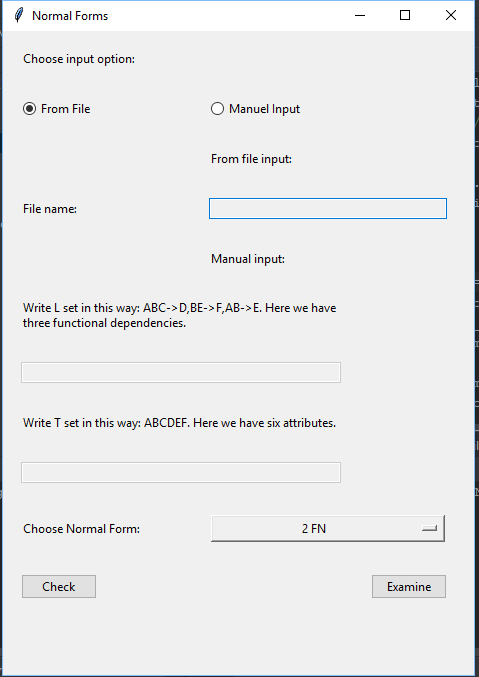
\includegraphics[width=0.3\linewidth]{Images/inicio.png}
  \caption{Inicio de la interfaz gráfica.}
  \label{fig:neurona1}
\end{figure}

Se observa que se tienen dos opciones para ingresar la información. La primera, es utilizando un archivo JSON. La segunda es ingresarla manualmente.

\subsubsection{Ingreso de relación por archivo JSON}
Para esto elegimos la opción del radiobutton "From File". A continuación damos clic en el botón "Examine". e obtendrá la siguiente imagen:

\begin{figure}[H]
\centering
  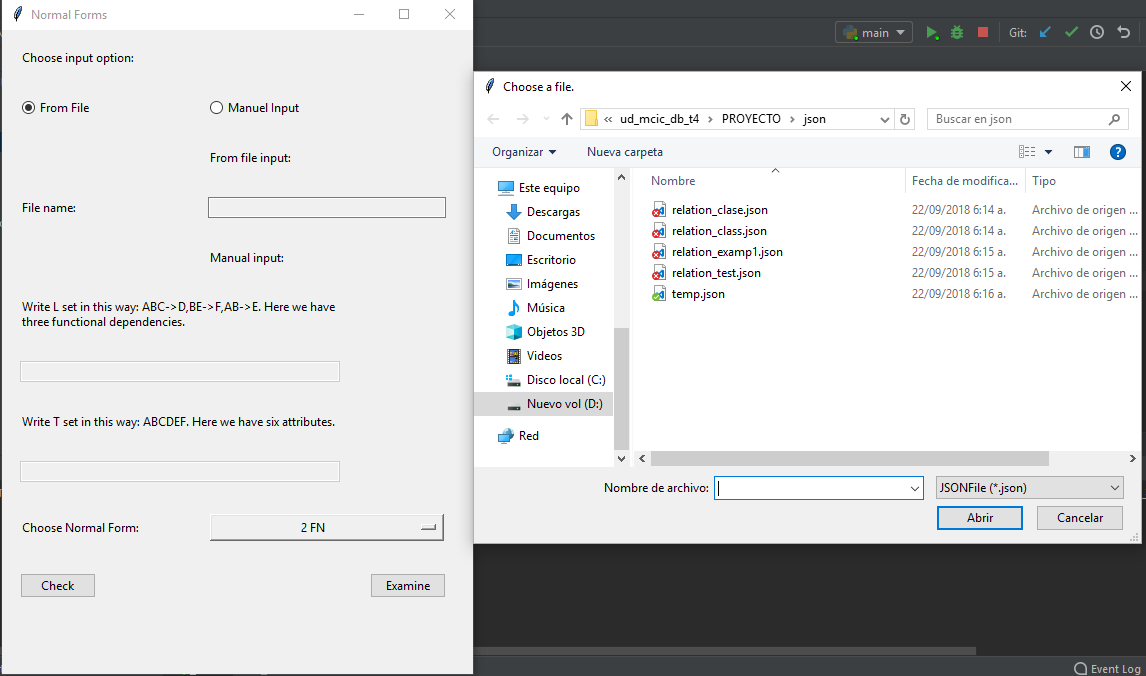
\includegraphics[width=0.75\linewidth]{Images/examine_file.png}
  \caption{Explorador de archivos.}
  \label{fig:neurona1}
\end{figure}

Al elegir un archivo, se verá la ruta completa en el cuadro de texto "File name:". Así:

\begin{figure}[H]
\centering
  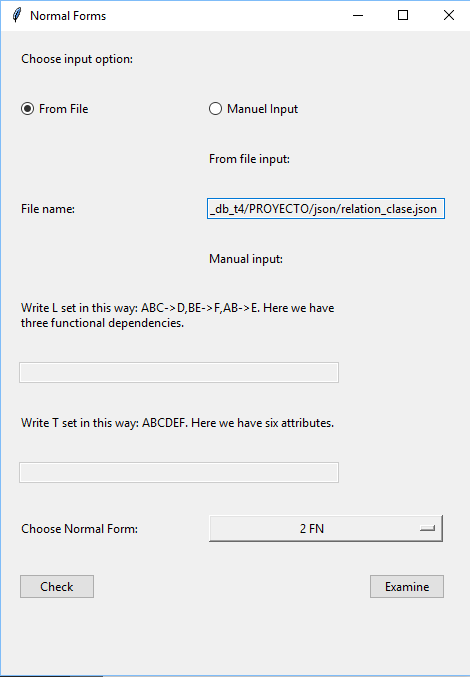
\includegraphics[width=0.3\linewidth]{Images/file_load.png}
  \caption{Archivo cargado.}
  \label{fig:neurona1}
\end{figure}


\subsubsection{Ingreso de relación de forma manual}

Para este caso, se debe ingresar la información manualmente. Primero debe seleccionarse la opción "Manual Input" del radiobutton.
\\
Deben seguirse las reglas indicadas en la interfaz gráfica. Esto es, ingresar los caracteres del conjunto de atributos $T$ en la caja de texto correspondiente.
\\
Estos deben ser un carácter en mayúscula por cada atributo. Deben ir pegados y estar en mayúscula. No hay importancia en su orden.
\\
Un ejemplo de esto se muestra a continuación:

\begin{figure}[H]
\centering
  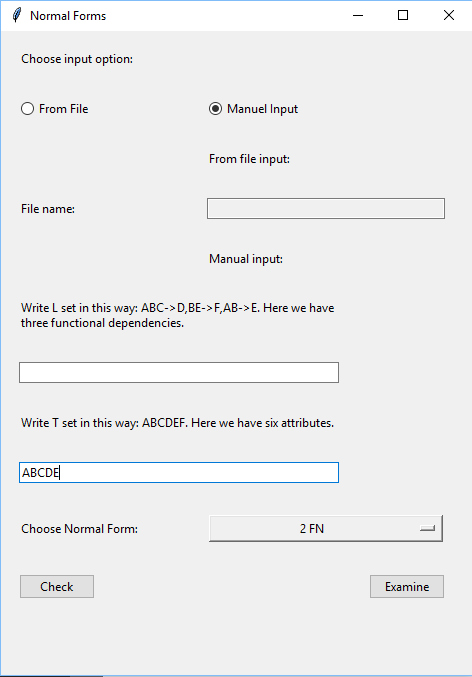
\includegraphics[width=0.3\linewidth]{Images/manual_tset.png}
  \caption{Conjunto de atributos ingresado manualmente.}
  \label{fig:neurona1}
\end{figure}

Para el caso del conjunto de dependencias funcionales $L$ deben ingresarse como parejas ordenadas, con el siguiente formato:

\begin{lstlisting}[language=python, caption={Ejemplo de dependencias.\\\hspace{\textwidth}}, captionpos=t]
ABC->E,EF->A,BD->C
\end{lstlisting}

Se entiende que hay tres dependencias funcionales, es decir:

\begin{enumerate}
\item ABC implica E
\item EF implica A
\item BD implica C
\end{enumerate}

El resultado en la interfaz gráfica se muestra en la siguiente figura:

\begin{figure}[H]
\centering
  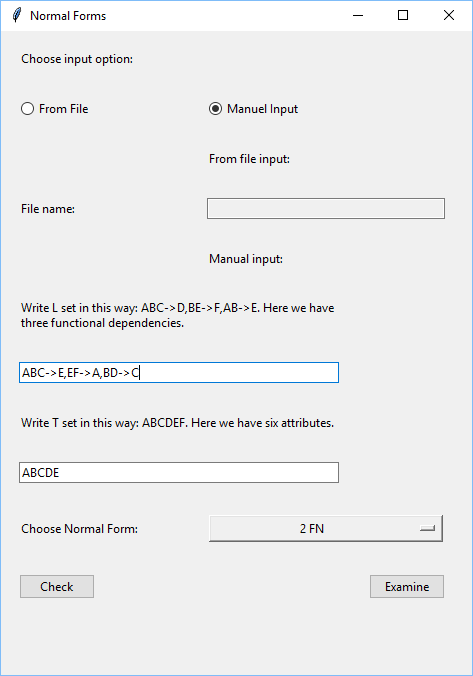
\includegraphics[width=0.3\linewidth]{Images/manual_lset.png}
  \caption{Conjunto de dependencias funcionales ingresado manualmente.}
  \label{fig:neurona1}
\end{figure}

Como se observa, en esta opción se tiene disponible el botón "Examine". Esto tiene como fin cargar los conjuntos desde un archivo JSON con el formato mencionado. Dicha información se pasará a las cajas de texto correspondiente.
\\
Esto se muestra en las siguientes figuras.

\begin{figure}[H]
\centering
  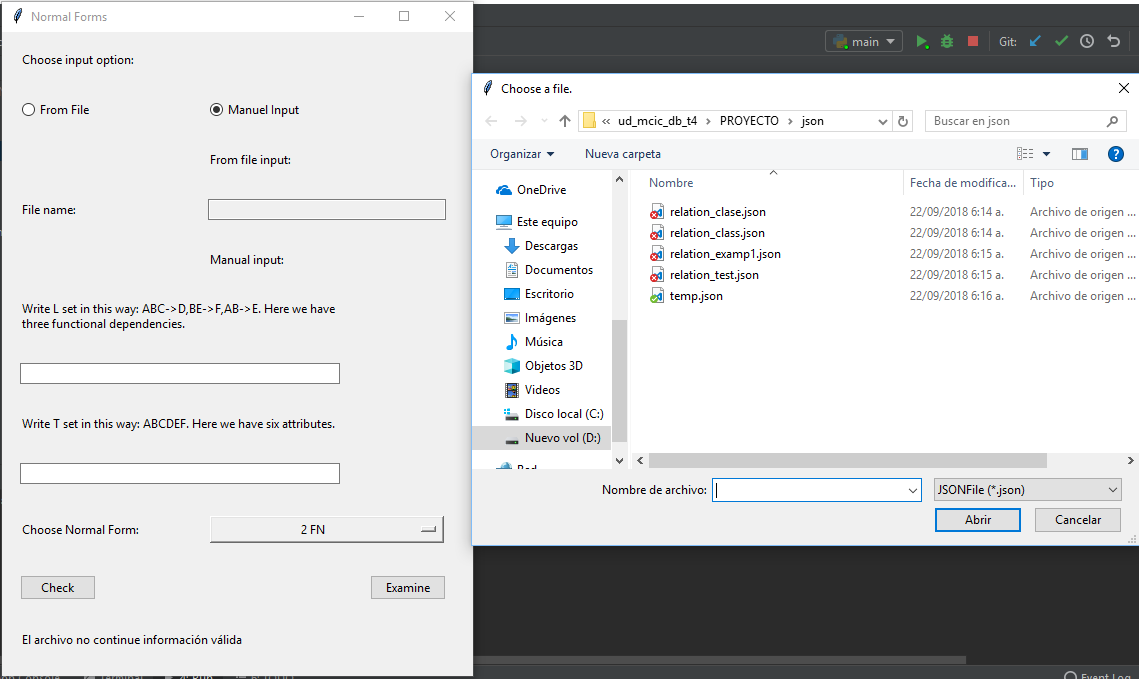
\includegraphics[width=0.75\linewidth]{Images/examine_manual.png}
  \caption{Explorador de archivos.}
  \label{fig:neurona1}
\end{figure}

\begin{figure}[H]
\centering
  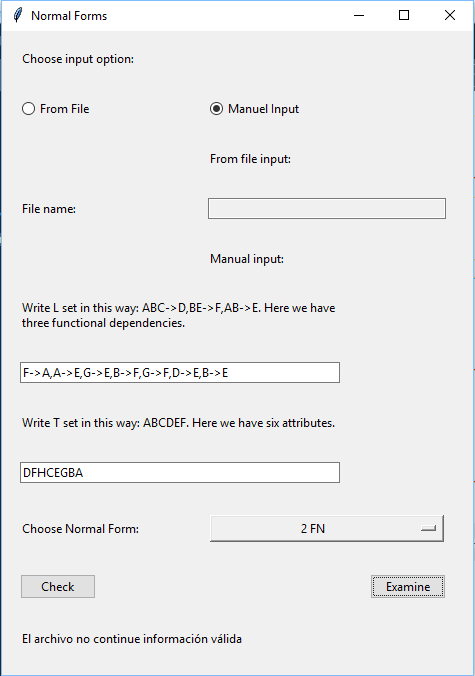
\includegraphics[width=0.3\linewidth]{Images/data_from_file.png}
  \caption{Datos cargados desde el archivo JSON a las cajas de texto.}
  \label{fig:neurona1}
\end{figure}



\subsubsection{Determinar formas normales}
Una vez de haya cargado la información (por cualquiera de los métodos mencionados), se debe elegir la forma normal que desea validarse del dropdownlist "Choose Normal Form".
\\
Esto se muestra en la siguiente figura:

\begin{figure}[H]
\centering
  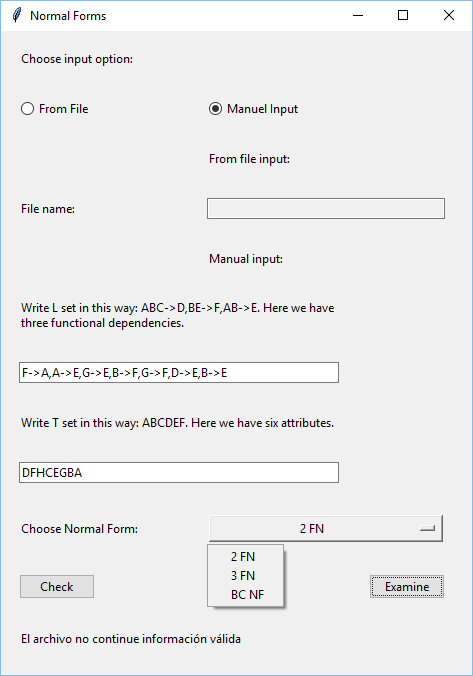
\includegraphics[width=0.3\linewidth]{Images/choose_nf.png}
  \caption{Selección de forma normal.}
  \label{fig:neurona1}
\end{figure}

Una vez seleccionada se da clic en check.
\\
Ejemplo de resultados se muestran a continuación:

\begin{figure}[H]
\centering
  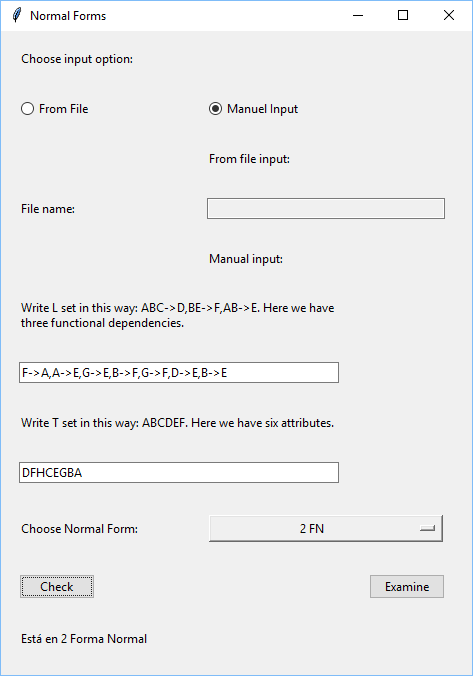
\includegraphics[width=0.3\linewidth]{Images/result_2nf.png}
  \caption{Resultado de la segunda forma normal.}
  \label{fig:neurona1}
\end{figure}

\begin{figure}[H]
\centering
  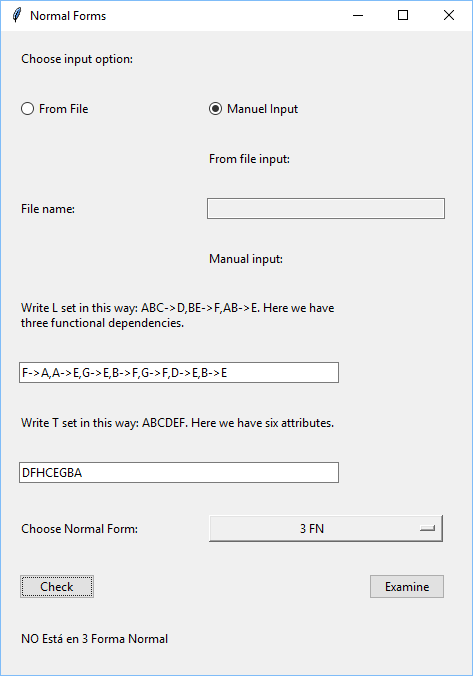
\includegraphics[width=0.3\linewidth]{Images/result_3nf.png}
  \caption{Resultado de la tercera forma normal.}
  \label{fig:neurona1}
\end{figure}

\begin{figure}[H]
\centering
  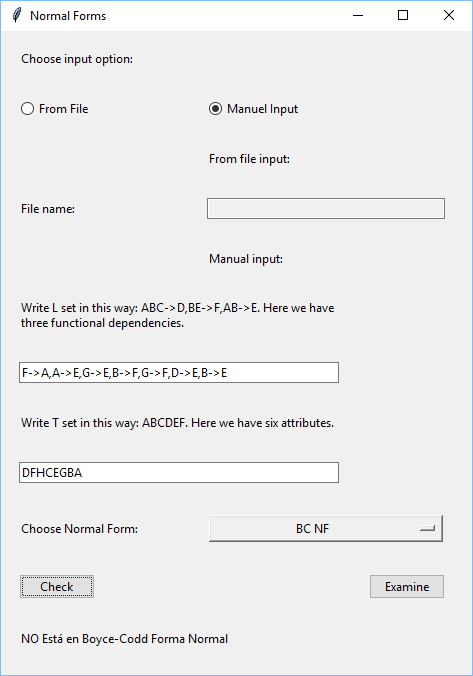
\includegraphics[width=0.3\linewidth]{Images/result_bcnf.png}
  \caption{Resultado de la forma normal de Boyce-Codd.}
  \label{fig:neurona1}
\end{figure}

\subsubsection{Repositorio}

Este proyecto estará en el siguiente \href{https://github.com/JoseManuelVargas/ud_mcic_db_t4}{\underline{Repositorio}}.

\newpage

\renewcommand\refname{Bibliografía}

%\begin{thebibliography}{9}

%\bibitem[A]{aligica} P.D. Aligica. \textsl{Julian Simon and the “Limits to Growth” Neo-Malthusianism}, Electronic Journal of Sustainable Development, \textbf{1}, 3, (2009), pp. 73-84. (http://goo.gl/23G1Oo)

%\bibitem[Au]{ausubel} J. H. Ausubel y P. S. Meyer. \textsl{Carrying Capacity: A Model with
%Logistically Varying Limits, Technological Forecasting and Social Change},
%\textbf{61}, 3, (1999), pp. 209-214. http://goo.gl/Lpc4g4

%\bibitem[Al]{alvarez} N. Álvarez-Vázquez, P.A. Pérez y J. Rodríguez-Ruiz. \textsl{Métodos y
%modelos matemáticos de la demografía}, (trabajo), Departamento de Economía
%Aplicada Cuantitativa, UNED, Málaga, 1997. http://goo.gl/n1Z2nM

%\bibitem[B]{bacaer} N. Bacaër. \textsl{A Short History of Mathematical Population Dynamics},
%Springer-Verlag, Londres, 2011. http://goo.gl/1LhzMB

%\bibitem[Ba]{banks} R. B. Banks. \textsl{Growth and Diffusion Phenomena: Mathematical
%Frameworks and Applications}, Springer-Verlag, Berlín, 1994.


%\end{thebibliography}


\end{document}



